\chapter{One Layer}
\label{chap:singleLayer}

{\em *** Version: \today~ ***}
\bc



Contents


Relation
lev low lev high

at element level 2 levels also relation

ES






TODO
check super & subscripts in figures and text: h/high h,trans or h_trans, etc.


IMPORTANT there seems to be an invariant that for a j:  i>j, all mappings are correct 
  ..           ...       
 .  .    ..   .   .   .. 
.    ....  ...     ...  .
 no it's not asymmetric. find out more about this.
 maybe it's just that a level is never presented twice without trans, and vice versa


SOMEWHERE: mappings important for extra state, but also for editing on several levels. (is this really true?)

RENDERER IS SPECIAL, LOWER THING IS NOT A TREE, EXPLAIN THAT THIS CHAPTER ONLY HOLDS FOR HIGHER LAYERS

MAPPING INFO INCONSISTENCY: figure out how to express that two cycles are needed to restore it.
                                                  %is probably related to edit ops starting at higher level
ALSO ALL IS ON TREES, for other things, eg, sum of leafs, it does not work, do it yourself
EXTRA STATE, also tree ordering? precedence op tree -> non ordered op tree?
SOMEWHERE, explain why this is all necessary, refer to Editing Chapter

No i's in this chapter!!! all is High and L Is this possible?

***EXTRA STATE is based on invariant mapping, however, implemented mapping is from level to level
***EXTRA STATE is only possible when inc. because lev, cannot be derived, or maybe only store extra?

** SOMEWHERE. pres is typically just for viewing: no big problem when destroyed
** trans is more essential. bigger problem when destroyed.
** guarantee no loss, so only limited edit func. on toc.

translation is bit strange as edit ops can be on higher level
* could this also be the case with presentation?



!!!!!!!!!
MAYBE we want to make Present and Translate the intended and specified mappings, 
without extra stuff and mappings, then the editor has to implement the incremental ones
 and mapping preserving things, so the result is that Present and Translate hold.

!however, in that case Present.Translate will not be id if Present is ambiguous, or 
has extra state. But maybe we don't care and only require the implementation to be id.

!what about sheets? 

SOMEWHERE: FOCUS more formally (if included then add forward refs to edit model chapter)


IMPL: mapping downward, how to store in doc? Now datatype changes when pres is modified

\ec

%provisional

%* explain edit steps? Before fitting it all together, we first build one layer

In the layered architecture of Proxima, each layer maintains invariants between two adjacent levels. When one level is changed, the adjacent level is updated in an appropriate way. Moreover, at each layer, the mappings in one direction turn out to be largely symmetrical to the mappings in the other direction.

This chapter discusses the invariants that are maintained between two adjacent levels, as well as the way in which the layer in between maintains the invariants by evaluating presentation and translation mappings. Furthermore, it specifies the additional information necessary for computing the layer mappings. The invariants given in this chapter holds for any layer in the Proxima system, although several layers will be simpler than the generic layer presented here.

% behavior is denoted with abstract, and then we give concrete functions that implement the abstract.

% next chapter, we connect everything.



% based on a mapping between levels
% add sheets, add extra and add incrementality

\note{Stress that mappings are not needed when for subtrees for which the lower level is not editable}
\note{Stress that it's only an architecture. Safety, impl. etc is left to layer. Future research (Pierce?)}
%rather than safe toy, complete arch for many ed's Safety and patterns need to be researched

\bc
Where say that mapping back is only when we need automatic editing: is it only important for duplicates? It seems to be important for 2:1 presentations as well.  In some complicated cases, the mapping back cannot be spec'd if mapping back is does not work, it means that lower edit cannot be handled, and is forbidden. However, we always have the higher level edit left.
\ec

%																
%																
%																
\section{The Presentation and Translation invariants}

% will become more a computation order

In order to relate the data levels surrounding one layer, we use two invariants: the {\em presentation invariant} and the {\em translation invariant}. The presentation invariant is satisfied if and only if the lower level is a correct presentation of the higher level. The invariant is expressed using an abstract function 
$Present ::  Level_{H} \rightarrow Level_{L}$.

\begin{small}\begin{math}
level_{L} = Present~level_{H}\\
%Present :: Level_{H} \rightarrow Level_{L} \\
\end{math}\end{small}

Similarly, the translation invariant is satisfied if and only if the higher level is a correct translation of the lower level. The translation invariant is expressed with the function 
$Translate ::  Level_{L} \rightarrow Level_{H}$.

\begin{small}\begin{math}
%Translate ::  Level_{L} \rightarrow Level_{H} \\
level_{H} = Translate~level_{L}\\
\end{math}\end{small}

The functions $Present$ and $Translate$ are abstract concepts used to express a property of two levels, not actual functions that can be evaluated. The functions are used specify the behavior of a layer.
Strictly speaking, $Present$ and $Translate$ are not even functions but relations, since a higher level may have several correct presentations, and a lower level may have several correct translations. However, this occurs only if a level has extra state, as will be explained in Section~\ref{sect:extraState}.

Because we only look at one layer in this chapter (ie. the layer between $Level_{H}$ and $Level_{L}$), we need two more functions to refer to the behavior of the layers below this layer, as well as the layers above. For lower layers, the function $Edit :: Level_{L} \rightarrow Level_{L}$ denotes an update on $Level_{L}$ by the lower layers. For representing updates on the higher level, we use 
$Transform :: Level_{H} \rightarrow Level_{H}$. In the next chapter, layers are connected, which removes the need for $Edit$ and $Transform$.

Figure~\ref{layerEditProcess} shows how the invariants can be used to specify the data level updates. The precondition before the edit operation takes place is that the lower level is a correct presentation of the higher level, that is $level_{L} = Present~level_{H}$. In the levels below, an edit operation takes place, which results in an updated lower level: $level'_{L}$. Because the presentation invariant will not necessarily hold anymore, an appropriate higher level is specified by the translation invariant:
$level'_{H} = Translate~level'_{L}$. The new higher level is then processed by higher layers, resulting in the final higher level value for this edit step: $level''_{H}$. Finally, the postcondition is established by updating the lower level to $level''_{L}$ for which 
$level''_{L} = Present~level''_{H}$ holds. 

The successive updates on the levels can be expressed with equations:

\begin{small}\begin{math}
level_{L} = Present~level_{H}\hfill \text{\{Precondition\}}\\
level'_{L} = Edit~level_{L}\\
level'_{H} = Translate~level'_{L}\hfill \text{\{Intermediate condition\}}\\
level''_{H} = Transform~level'_{H}\\
level''_{L} = Present~level''_{H}\hfill \text{\{Postcondition\}}\\
\end{math}\end{small}

% also do an EDIT condition that says the new thing is what we intend with the 
% edit gesture? Does not seem to make sense for a single layer. Maybe do it in the % next chapter

% can we express when this happens with a condition? pres .. /= pres .. oid?
The reason why $level'_{H}$ is not immediately presented, is that it has to be processed by the higher layers, just as $level'_{L}$ is processed by this layer. The final value $level''_{H}$ may be equal to $level'_{H}$, but this is not always the case. Take, for example, an enriched document that contains a list of numbers together with the sum of the numbers. When one of the numbers is edited on presentation level, the new enriched document that results from parsing ($level'_{H}$) is a list of numbers together with a sum value that might not be correct anymore. In order to get the correct value, the enriched document is passed on to the reducer and evaluator, resulting in a final enriched document ($level''_{H}$) that contains a correct sum.

\begin{figure}
\begin{small}
\begin{center}
\begin{center}
\epsfig{file=pics/eps/layer.eps, height=1.7in} %, width=80mm}
%\begin{small}
%\xymatrix{
%                      \ar@{.>}[d] &  &                       \ar@{.}[rr] & &                   \ar@{.>}[d]  \\
% \data{$level_{H}$} \ar[d]     &  & \data{$level'_{H}$} \ar@{.}[u] & & \data{$level''_{H}$} %\ar[d] \\ 
% \component{$Present$} \ar[d]     &  & \component{$Translate$} \ar[u]    & & \component{$Present$}  %\ar[d]  \\
% \data{$level_{L}$}  \ar@{.}[d] &  & \data{$level'_{L}$}  \ar[u]     & & \data{$level''_{L}$} %\ar@{.>}[d]\\
%                      \ar@{.}[r] & \abscomponent{User Edit} \ar@{.}[r]  &                      \ar@{.>}[u]  & &         %                       \\
% {\rm Precondition}               &  & {\rm Intermediate~condition}      & & {\rm Postcondition}            \\
%}
%\end{small}
\end{center}\caption{An edit step on one level.}\label{layerEditProcess} 
\end{center}
\end{small}
\end{figure}

% why two:
We have to use two invariants instead of one, to make it possible to distinguish between the intermediate condition and the postcondition. The alternative would be a single invariant, stating that the lower level is a presentation of the higher level, as well as that the higher level is a translation of the lower level. However, now we cannot express the situation that a higher level is a correct translation of a lower level, without this lower level being a correct presentation of the higher level.

% example of this
As an example, consider an editor in which an enriched document node \verb|Plus (Int 1) (Int 2)| is presented as a list of presentation level tokens, colored according to the syntax. The integer values are presented in black, and the operator in green. If we denote a token as a string value with a color in between braces, the presentation is \verb|["1" {black}, "+" {green}, "2" {black}]|. Because the presentation level is a correct presentation of the document level, the presentation invariant is satisfied. But now consider a list of tokens typed by the user, which do not have the correct coloring: \verb|["1" {black}, "+" {black}, "2" {black}]|. If we want to be able to express with only one invariant that the enriched document \verb|Plus (Int 1) (Int 2)| is the appropriate translation of this list, then the uncolored sequence must also be a correct presentation of the sum. Hence, with a single invariant, we cannot express that in the final state the colored presentation is a correct presentation of the sum, whereas the uncolored presentation is not. \note{are we saying that with one invariant, pres is inverse of trans?}


%\note{mention that these things need to be each other's inverse}
%******** NOT TRUE, this will appear somewhere more downward, probably in ES section
%The functions $Present$ and $Translate$ are closely related, but in contrast to what the types might %suggest, the functions are in general not each others inverse. Because translating a presented document %should not change the document, we do have: 
%
%\begin{small}\begin{math}
%Translate \cdot Present = id_{H}
%\end{math}\end{small}
%
%\note{what about ambiguity?}
%
%However, the reverse ($Present \cdot Translate = id_{L}$) does not necessarily hold. The condition %implies that an edited lower level does not change when it is translated and presented \note{also say that %higher layers should not change it?}, which is not always true. The syntax coloring example provides a case %in which it does not hold; if an uncolored presentation is translated and then presented, the result is a %colored presentation. 
%\note{pres is injective, and trans isn't?}

%summary
Summarizing, the $Presentation$ invariant specifies that two levels are in a final state, in which the lower is a correct presentation of the higher. When the lower level is updated, the $Translation$ invariant specifies a correct new higher level, which is passed on to the higher levels. The higher levels return a final for this edit step value for the higher level, for which a correct final lower level is specified by the $Presentation$ invariant. The layer in between each pair of levels takes care of maintaining the invariants, by invoking functions that establish the presentation and translation invariants.

\note{say something about Translate.Present here as well?}

\bc
?present~sheet~.~translate~sheet = id_{H}\\

OTHER EXAMPLE?: Apart from the syntax coloring example, the problem also arises when for example a textual arrow 
\verb|"->"| is presented as a $\rightarrow$. In that case, a lower level containing textual arrows is 
translated on a higher level 

Vice versa? Fix by remembering extra?
 layer shortcutting can now be expressed by only letting the lower pres invariants hold

 -explain that in incremental, present and translate cannot be used instead of Present and Translate
 -how does this relate to inc with diff etc. maybe that can be expressed nicely with Present
 (or even present, then Present will be superfluous.)

* does   trans.pres = id hold for a layer? pres.trans never needs to hold due to syntax coloring, normalization etc., but also because Chess board is not a presentation of ChessBoard   
* trans.pres = id? then each pres has unique doc. Is this true? Can't doc variants be presented as same thing?
   present( translate uncolored ) = colored, so present.translate /= id
   translate ( present ) = id? if so, what if two docs are presented on the same pres?
 it seems true, translate.present cycles should not alter the doc. In case of ambiguity, the system should
 take care of conservative behavior. On an edit, the doc may change, but that's not a (translate.present) cycle


 ****** When this is figured out, update sheet paragraph
\ec


%																
\subsection{Upward and downward mappings at one layer} \label{mappingsInLayer}

% mapping is relation levelH levelL but each two levels express a mapping between nodes.

During presentation and translation, elements in one data level are mapped onto elements in another level. Hence, when either the presentation or the translation invariant holds between two levels, we also have a mapping between the tree nodes of these levels. 

Figure~\ref{nodeMapping} shows an example of such a mapping between two levels. The dotted arrows denote on which lower level nodes a higher level node is mapped and vice versa. To reduce the number of arrows in the figure, the lower level nodes are grouped.

\bc The presentation and translation invariants are expressed using two functions\note{incorrect:relations}: $Present$ and $Translate$. The functions are of type $Level_i \rightarrow Level_j$ (where $j = i+1$ or
$j = i-1$), which means that both functions map a tree onto another tree. However, since a tree structure consist of nodes, we can also view each mapping as a mapping between the nodes of one tree and the nodes of another tree. \note{do we put a restriction on the possible mapping functions with this?} 
\ec

By mapping between tree nodes, we mean a mapping that relates only the nodes, and not the subtrees rooted at theses nodes. We can see this in Figure~\ref{nodeMapping}, by the fact that a child of a lower level node is not necessarily inside the same dotted ellipse as its parent.

A difference between the presentation and translation mappings, is that a higher level node may be presented onto several lower level nodes, whereas a lower level node may be translated on only one higher level node. This is why the nodes on the right side (the lower level) are grouped together with dotted ellipses, whereas the nodes on the left side are not. The reason for the distinction is that 
\toHere     % ^^^^^^^^^^^^^^^^^^^^^^^^^^^^^^^^^^^^^

% restriction is on presentation. pres is like a fold
% iets algemener verhaaltje hier. over dat het wel kan, maar dat de
% automatische dingen (focus etc.) dan weg zijn

WHY this restriction? AG automatically does this, but do we need to enforce? What about focus, is that the reason?
Difference between pres and trans. Beetje lastig omdat pijlen in plaatje maar 1 kant opgaan.
**
\toHere     % ^^^^^^^^^^^^^^^^^^^^^^^^^^^^^^^^^^^^^


\bc
Hence, when an element \verb|A| is mapped onto an element \verb|B|, this does not say anything about the children of \verb|A| and \verb|B|. If \verb|A| is mapped onto \verb|B| including its children, this is mentioned explicitly. In Figure~\ref{nodeMapping} element \verb|aH| is mapped onto the elements \verb|a1L|,\verb|a2L|, and \verb|a3L|, so in this case the children of \verb|a1L| are included in the mapping, but the children of \verb|a2L| and \verb|a3L| are not. 
\ec

\bc
When regarded as relating tree nodes, a mapping can express an $n:m$ relation between the nodes of the higher and the lower levels. However, when regarded as relating levels, a mapping is always a function (ie. an $n:1$ relation). Thus, $Present$ and $Translate$ are functions rather than relations.
\note{WITH ES, they are relations!}
\ec

\begin{figure}
\begin{center}
\begin{center}
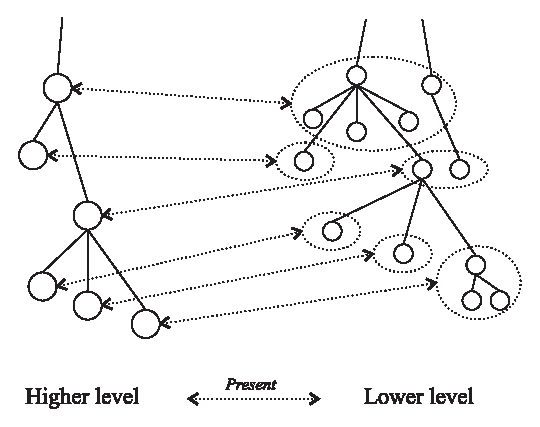
\epsfig{file=pics/eps/mapping.eps, width=2in}
%\begin{verbatim}
%
%     aH        higher level
% bH      cH
% 
%
%                    Layer
%
% 
%     a1L 
% a2L         a3L   Lower level
% bL         cL
%\end{verbatim}
\end{center}
\caption{A mapping between the nodes of two levels.}\label{nodeMapping} 
\end{center}
\end{figure}

\bigskip {\bf The presentation mapping}

\begin{figure}
\begin{center}
\begin{center}
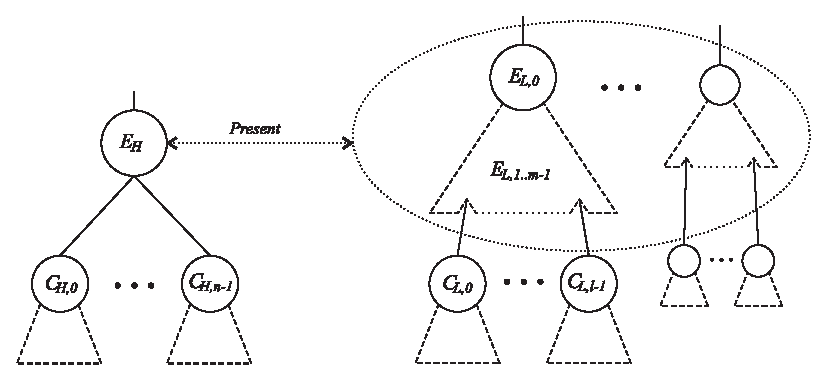
\epsfig{file=pics/eps/presentationEh.eps, width=2in}
%\begin{verbatim}
%                  ..
%                    \
%..                   EL0
%  \                 ELEL.
%   EH       ->     EL..EL.
%  / \             EL....EL. 
% C...C           EL......EL.
%                EL/\EL.EL/\EL.
%                 /__\   /__\
%                    
%\end{verbatim}
\end{center}
\caption{The presentation of element $E_H$.}\label{elementPresentation} 
\end{center}
\end{figure}

First we take a closer look at the downward, or presentation, direction. $Present$ maps each element of the higher level onto zero or more lower level elements, forming zero or more subtrees with holes. \note{is there a name for 'tree with holes'? eg. 'tree segment'?} Figure~\ref{elementPresentation} shows the presentation of one node ($E_H$) in the higher level. $E_H$ is an element in the higher data level that has $n$ children ($C_{H,0}$, \dots, $C_{H,n-1}$). The presentation of $E_H$ is a number of trees (although usually just one) that may consist of several nodes. In the figure, the first tree is shown in more detail. It consists of $m$ nodes is rootet at $E_{L,0}$. 

The $C_{L,0}$, \dots, $C_{L,l-1}$ subtrees in the lower level tree are not part of the presentation of $E_H$. Typically, these are the presentations of the children of $E_H$, but in general they can be (part of) the presentation of any element in the higher level. Alternatively, if a subtree is not part of the presentation of any higher level element, it is part of the extra state of the lower level, which is explained in the next section.

\begin{figure}
\begin{center}
\begin{center}
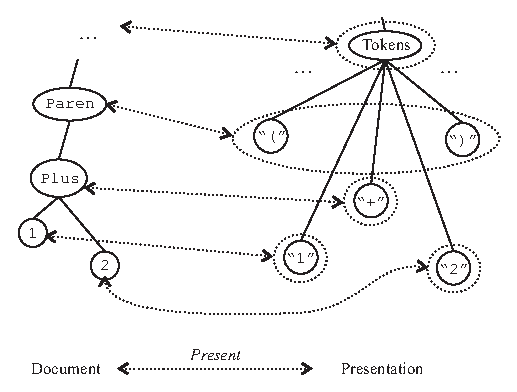
\epsfig{file=pics/eps/presentParenSum.eps}
%
%  ( )       Tk   ( 1+2 )
%   +      Tk ...
%  1 2       .....  
%
\end{center}
\caption{The presentation of a parenthesized sum.}\label{presentExample} 
\end{center}
\end{figure}

Figure~\ref{presentExample} provides a more concrete example of a presentation, taken from a source editor. A parenthesized sum in the enriched document is presented as a set of tokens on the presentation level. The figure shows only a fragment of the enriched document and its presentation. \bc , leaving out the tokens to the left and the right of the expression, as well as the origin of the Tokens element. \ec The tuples in the presentation represent the whitespace of the tokens (line breaks, spaces) as defined in Section~\ref{sect:presLevel}. To the editing user, the expression will be appear as "{\tt (\textvisiblespace 1+2\textvisiblespace )}". The tuples lie outside the dotted ellipses because white space is extra state of the presentation level (see Section~\ref{sect:extraState}). 

\bc
In the example, the resulting presentation is a single tree, but this is not always the case. For example, the evaluation layer in a word processor (see Section~\ref{sect:wordprocessor}), maps each chapter onto an entry in the table of contents, as well as onto the presentation of the chapter itself. Hence, the presentation (in this case the evaluation) of a chapter consists of two separate enriched document trees.
\ec

\bigskip {\bf The translation mapping}

The upward direction, or translation, is slightly more restricted than the downward direction, because a lower level element is allowed to be mapped onto at most one higher level element. Figure~\ref{elementTranslation} schematically shows a translation of a numebr of subtrees rooted at $E_L$. The children in the lower level tree are not mapped onto $E_H$, but may be mapped onto its children (or they may be ignored in the mapping).  Again, the lower level structure is not necessarily a single subtree (with holes); it may consist of several subtrees, e.g. when three presentation tokens \verb|"if"|, \verb|"then"| and \verb|"else"| are mapped onto an \verb|If| node in the enriched document in the parsing phase.


\begin{figure}
\begin{center}
\begin{center}
\epsfig{file=pics/eps/translationEh.eps, width=2in}
%\begin{verbatim}
%
%        EL                 ->    EH
%    EL.......EL               CH ..  CH
% EL  CL  EL  CL  EL
%
%\end{verbatim}
\end{center}
\caption{The translation of the tree rooted at {\tt EL} (beetje dubbel?)}\label{elementTranslation} 
\end{center}
\end{figure}

A consequence of the difference between the presentation and the translation mappings is that even when a lower level element depends on several higher level elements, only one is responsible for its presentation. For example when an element \verb|Word Color String|, representing a colored string, is presented as a string in the specified color. Now the string in the presentation . In order to edit the color

  \note{where does this become important?} \note{example: leaf Color Int $\rightarrow$ colored int. When selecting, either lead or int,  Color affects but is not responsible. can be accessed by special edit ops though.}
\note {maybe say something about 1:n presentation restriction, but also about having $>$1 doc nodes influence same pres.? Or before?}


******** BIG PROBLEM With IntExp  Int. 
Is IntExp translation ES (Then ES is not always a subtree, but can be a segment as well: Paren -- IntExp(es) -- Int )? Then reusing is not as easy anymore.
Or can we translation map onto 2 nodes after all?
Or do we just ignore elts with no pres and rebuild them when translating?

NEED MORE EXPERIENCE!!

%\toHere     % ^^^^^^^^^^^^^^^^^^^^^^^^^^^^^^^^^^^^^
%
%
%*what about parsing to something double?
%*what about IdExp (Id "a")    ->   "a"
%*Isn't this too restrictive?
%* doesn't this make the presentation more simple? translation is hard because several elements need to be 
%regarded.
%if we propagate a value downward as an attribute, it already happens.
%\fromHere  % VVVVVVVVVVVVVVVVVVVVVVVVVVVVVVVVVVVVVVVVVVVV


%* if then else? tokens as list? then focus does not work (no?). tokens as tree?

\bigskip {\bf Duplicates in presentation}
\fromHere  % VVVVVVVVVVVVVVVVVVVVVVVVVVVVVVVVVVVVVVVVVVVV

\note{mention duplicates in translation?}

%* not just because multiple trees: elements may depend on several trees. without duplication.

The presentation of a higher level element may consist of several lower level elements, for example when an \verb|If| node is presented with three tokens. In this case, the three tokens together are translated to the \verb|If| node. However, it is also possible that an element is duplicated in the presentation, in which case two (or more) lower level structures  translate to the same higher level element, possibly creating a conflict. An example of such a copy is the title of a chapter that appears in the table of contents as well as in the presentation of the chapter itself. When the lower level is translated, several alternatives for one element may arise, and a choice has to be made. 
\note{hard to express this as a mapping}

Note that having several lower level elements does not automatically mean that an element is duplicated. The  \verb|If| node is presented on three tokens, but this does not constitute a duplication. Furthermore, translation of duplicates only needs to be dealt with if the duplicate structure is edited on the lower level. If a duplicate only needs to support document editing and no presentation editing, no extra work needs to be done.

The only two layers in which duplicates can be created are the evaluation and the presentation layer. The presentation mappings for the other layers are largely predefined and do not duplicate any structures. To avoind having to deal with duplicates when parsing, duplicating is allowed only at the evaluation layer. This restriction may be lifted in a future version, but for now, if a presentation contains duplicates, the evaluation sheet specifies how the involved structures are duplicated, and the reduction sheet specifies how updates on duplicate structures are handled.

\begin{figure}
\begin{center}
\begin{center}
\epsfig{file=pics/eps/translateToc.eps}
%
%  Chap              Toc
%  "first.."     TokChap      Chap
%                   "first.."     "first.." 
%
\end{center}
\caption{The translation of a word processor document with a table of contents.}\label{translateExample} 
\end{center}
\end{figure}

Figure~\ref{translateExample} shows an example of a duplicated structure in the form of a table of contents for a word processor. On the lefthand side of the figure is a document that contains two chapters, of which only the titles are shown. The enriched document contains both a table of contents tree (\verb|Toc|), as well as a copy of the chapters. The table of contents tree follows the structure of the document, but only contains the title of each chapter rather than the chapter itself. To keep the figure simple, the table of contents only contains chapters and not sections and subsections, but in a real editor the table of contents may reflect the entire document structure. 

The evaluator maps a chapter in the document on a chapter in the enriched document, as well as on a chapter entry in the table of contents tree, leaving out everything but the title in the latter case. The presenter simply presents both the table of contents tree as well as the chapter tree, and does not duplicate any structures. The table of contents example is somewhat complex, because it does not only involve a duplicated presentation, but also a partial presentation (a chapter in the table of contents is shown without its content). Section~\ref{sect:extraState} discusses how partial presentations are handled.

When the enriched document is edited, it is translated (reduced) to an updated document. For duplicate structures, the enriched document contains several alternatives, which may have different translations. In the table of contents example, the alternatives for a chapter title are the title in the table of contents and the title in the chapter. Three situations are possible. Firstly, if none of the alternatives has been edited, all alternative values translate to the same document value, so any one can be chosen. Secondly, if one alternative has been edited, the choice is in favor of the edited element. Hence, if a chapter title is edited in the table of contents, the resulting reduced document contains the updated title. Finally, if more than one value has been edited, an error is signaled to the user. In the example, this happens when the title is edited in the chapter as well as in the table of contents. In this case the edit operation may be forbidden, or one of the values may be chosen.  \note{say that we cannot skip the evaluation layer with this scheme}

Specifying duplications in the evaluation and reduction sheets is not ideal, since the enriched document type now depends on whether or not the presentation contains duplicates. Hence, if a presentation contains several views on a structure, the necessary duplications for these views need to be specified in the evaluation layer. A special facility in for specifying common duplicate presentations, such as tree views on a structure, in the presentation layer is desirable. A possible approach for such functionality is a special parser that can resolve conflicts duplicates during parsing. With such a parser, the whole process of handling duplicates takes place in the presentation layer, and the evaluation layer is not affected. \note{parse (dirty arrangement) $\rightarrow$ dirty presentation? May be tricky as well}

%																
%																
%																
\section{Extra state} \label{sect:extraState}

%SOMEWHERE: when es is hard. If no parent with a presentation is parent then 
% tricky. Hence invisible elements with extra state may lose it during editing.

\note{specify conditions for safety? like in Pierce's lenses stuff?}
\note{mention Pierce paper}

\toHere     % ^^^^^^^^^^^^^^^^^^^^^^^^^^^^^^^^^^^^^

The equations from the previous section assume that a level can be computed from the old values for the two levels together with a sheet and an edit operation on one of the levels. However, this turns out not to be entirely true in the presence of {\em extra state} (also see sections~\ref{sect:editingExtraState}~and~\ref{sect:archExtraState}). If we consider two adjacent data levels, some elements in one level cannot be derived from the other level. 

**
Figure~\ref{layerExtraState} shows two examples levels with the presentation mapping expressed with arrows. The shaded nodes on the higher level have no presentation elements and hence cannot be computed from the lower level during translation. Such elements that cannot be computed from the other level, are referred to as extra state elements.  \note{explain dependency on direction already here?}

% also show a vice versa? with two invariants, it's maybe not logical to show both in one figure

% This is still a copy of  \ref{nodeMapping}
%
\begin{figure}
\begin{center}
\begin{center}
\epsfig{file=pics/eps/prestransESExamples.eps, width=4in}
%\epsfig{file=pics/eps/2levelES.eps, width=4in}
%\begin{verbatim}
%
%        aH        higher level
%  bH         cH
%<shaded>
%
%                    Layer
%
% 
%     a1L 
%          a3L   Lower level
%          cL
%\end{verbatim}
\end{center}
\caption{Two examples of extra state.}\label{layerExtraState} 
\end{center}
\end{figure}
%CAPTION: shaded is extra
%PLAATJE figure of level with arrows, that contains extra state


%This section gives a more precise definition of extra state and specifies how  Furthermore, 
%This section explains : welke info. wanneer gaat het mis. 


%																
\subsection{Extra state in presentation and translation direction}

% One layer: two kinds of extra
Since a presentation of an element may consist of zero or more elements, and a translation consists of at most one, it is possible that an element is not mapped onto any elements in the other level. In that case, the other level simply does not contain the information needed to compute the element, and hence it is part of the former level's extra state. Because the property of extra state depends on the direction of the mapping, we distinguish two kinds of extra state: presentation extra state and translation extra state. The {\em presentation extra state} consists of elements that during presentation cannot be computed from the higher level (the shaded elements at the top level of Figure~\ref{layerExtraState}), and the {\em translation extra state} consists of elements that during translation cannot be computed from the lower level (the shaded elements at the bottom layer of the figure).

% example pres extra
An example of presentation extra state is the whitespace information of a token at the presentation level. This information is not present in the enriched document layer. Instead, the information is reused from the previous presentation of the enriched document. During presentation, tokens are reused, causing the whitespace information to stay the same. In order to do this, we need to know exactly on which presentation elements an enriched document node is mapped in the previous presentation.

% example trans extra
A word processor with an editable table of contents view provides an example of translation extra state.  For sake of simplicity, we will assume that the enriched document only contains the table of contents and not the chapters themselves. This way, we only have to consider the extra state here and not the duplication. Section~\ref{mappingsInLayer} already showed how handle duplications in general, and the same method can be used for the table of contents. 

The evaluator maps chapters, sections, and subsections in the document onto entries in the table of contents tree. An  entry does not contain the content of the corresponding document section, but only its title and entries for its children. During reduction, the table of contents is mapped back onto a complete document, including the parts that are not present in the enriched document. The title of a section comes from the table of contents entry enriched document, but the missing section content is obtained mapping an entry back onto the section that was mapped onto it during the evaluation phase. The section contents, as well as any other child elements that are not in the table of contents, are translation extra state of the evaluation layer.
 
\note{mention that trans ES is more important then pres ES here?}

% even with pres, there can still be extra state
Even if an element \verb|X| is mapped onto one or more elements \verb|Y|$_n$  in the other level, it can still be part of the extra state, if the elements \verb|Y|$_n$ do not constitute enough information to be mapped back onto \verb|X|. Consider for example a presentation of a Haskell source, in which al integers are presented with the string \verb|<Int>|. The integer nodes do have a presentation, but since it does not contain enough information for the backward mapping, the integer nodes are in translation extra state. \note {Is this also the case for focus} \note{Don't know much about this kind of ES yet}
%%%

An important point to note is that extra state with regard to a certain mapping, is extra state for the {\em result} type of the mapping. Hence, presentation extra state for a presentation mapping between $Level_{H}$ and $Level_{L}$ is part of $Level_{L}$. Although the term presentation extra state of $Level_i$ may suggest that this concerns state that is used during the presentation of $Level_i$, this is not the case. The extra state of $Level_i$ refers to the extra state with regard to the presentation of the level above ($Level_{i-1}$) on level $Level_i$. The only extra state that involved in the presentation of $Level_i$ is that of its lower neighbor: $Level_{i+1}$



%																
\subsection{One level has two kinds of extra state}

% One level: two kinds of extra
Figure~\ref{layerExtraState} only shows one layer, but since each data level except the document and the rendering is in between two layers, each level between the document and the rendering has two kinds of extra state. Figure~\ref{levelExtraState} shows a data level between two layers. In the figure, both the shaded elements and the bold elements are extra state. The shaded elements are presentation extra state with regard to the higher level, and the bold elements are translation extra state with regard to the lower level. Extra state in one direction is independent of extra state in the other direction, hence an element in the figure can be shaded, bold, shaded as well as bold, or neither. 

\begin{figure}
\begin{center}
\begin{center}
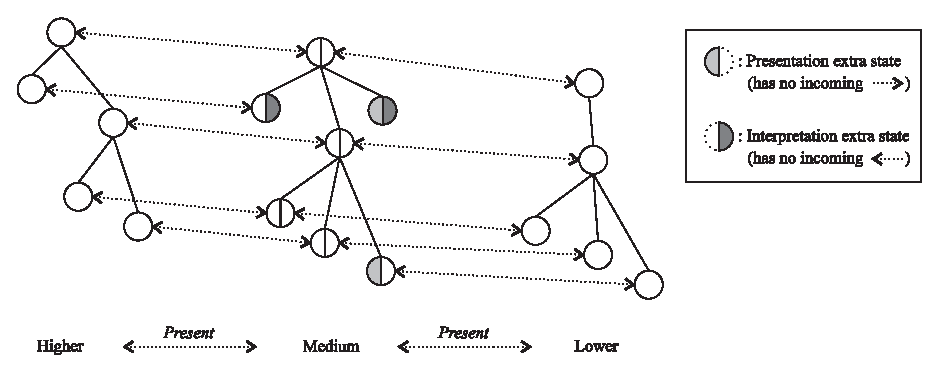
\epsfig{file=pics/eps/3levelES.eps, width=5in}
%\begin{verbatim}
%Level                elt   elt
%                         v    v 
%Level    shaded  elt  bold
%               ^        ^
%Level       elt      elt
%\end{verbatim}
\end{center}
\caption{Presentation and translation extra state in one level.}\label{levelExtraState} 
\end{center}
\end{figure}

% example one level independence of es
The whitespace extra state in tokens provides an example of the fact that the property of extra state in one direction is independent of extra state in the other direction. When the scanner layer translates the layout level, spaces and row transitions between a token's string and the preceding token's string are encoded as whitespace information in the token. Since it can be computed during translation, the whitespace is not part of the translation extra state. On the other hand, when the enriched document is presented on tokens in the presentation level, the whitespace information cannot be computed, and hence it is part of the presentation extra state of the presentation level.
 
\note{also example of one level with both kinds of extra state? Will be somewhat contrived}
%Example Decl, Decl Type Exp., Tree view
%So always Info Pres and Trans. bla core extra:


% equations:
More formally, a data level ($Level_{i}$) can be considered either as the product of the presentation extra state ($Extra_{Pres,i}$) and non-extra state ($Core_{Pres,i}$), or as the product of the translation extra and non-extra state ($Extra_{Trans,i}$ and $Core_{Pres,i}$). The document ($Level_0$) and the rendering ($Level_n$) are special cases, since the document has no presentation extra state, and the rendering has no translation extra state. Expressed with equations, we get:

% Note that pres es for level i is important for pres of level i-1
% and trans es for level i is important for trans of levl i+1
\begin{small}\begin{align*}% \label{sse}
\end{align*} 
\begin{math}
Level_{0} = Core_{Trans,0} \times Extra_{Trans,0}
Level_{n} = Core_{Pres,n} \times Extra_{Pres,n}
\forall 1 \le i \le n-1:  \\
Level_{i} = Core_{Trans,i} \times Extra_{Trans,i} = Core_{Pres,i} \times Extra_{Pres,i} 
%\\
%Present_{i} :: Level_{i} \rightarrow Core_{Pres,i+1} \\
%Translate_{i} :: Level_{i+1} \rightarrow Core_{Trans,i} \\
\end{math}\end{small}


%																
\subsection{Mapping information}

for reuse, need mapping info. both dirs. it is the arrows from bla.

% what extra info to keep
The $Extra$ information in the result types cannot be computed from the arguments. Instead, we try to reuse its previous value. In order to do so, ${\tt translate}$ and ${\tt present}$ get an extra argument which, for each node, contains the nodes it was previously mapped onto. For ${\tt translate}$, the extra argument is of type $Info_{Trans}$, and it is computed by ${\tt present}$. Analogously, ${\tt present}$ gets an extra argument of type $Info_{Pres}$, which is computed by ${\tt translate}$. \note{already mention computation order here?}


Except for the top and bottom levels, all levels contain presentation and translation information. The top level is never the result of a presentation mapping, and hence has no presentation information, whereas the bottom level has no translation information. The definition of $Level_i$ and the types of $present_i$ and $translate_i$ become:

\begin{small}\begin{align*}% \label{sse}
\end{align*} 
\begin{math}
Level_{0} = (Core_{Trans,0} \times Extra_{Trans,0}) \times Info_{Trans,0}\\
Level_{n} = (Core_{Pres,n} \times Extra_{Pres,n}) \times  Info_{Press,n}
\forall 1 \le i \le n-1:  \\
Level_{i} = (Core_{Trans,i} \times Extra_{Trans,i}) \times Info_{Pres,i} \times  Info_{Trans,i}\\  
               = (Core_{Pres,i} \times Extra_{Pres,i})  \times Info_{Pres,i} \times  Info_{Trans,i}\\  
\\
translate_{i} :: sheet_{Trans} \rightarrow Level_{L} \rightarrow Level_{H}\\
present_{i} :: sheet_{Pres}  \rightarrow  Level_{H} \rightarrow Level_{L}\\
\end{math}\end{small}



\bc
\begin{small}\begin{align*}
translate_{i} :: sheet_{Trans} \times Info_{Trans,L} \rightarrow Level_{L} \rightarrow Core_{Trans,H}  \times Extra_{Trans,H}  \times Info_{Press,H}\\
present_{i} :: sheet_{Pres}  \rightarrow Info_{Pres,H} \rightarrow  Level_{H} \rightarrow Core_{Pres,L} \times Extra_{Pres,L}   \times Info_{Pres,L} \\
%\\
%level'_{H} = {\tt translate}~sheet_{Trans}~info'~level'_{L}\\
%level''_{L} = {\tt present}~sheet_{Pres}~level''_{H}\\
%\\
%Present_{i} :: Level_{i} \rightarrow Core_{Pres,i+1}\\
%Translate_{i} :: Level_{i+1} \rightarrow Core_{Trans,i}\\
\end{align*} 
\end{small}
{\centering ()\\}


% example in picture 
Figure~\ref{mappingInfo} shows two examples of the $Info$ argument. The lefthand side shows the situation at the presentation layer of a Haskell source editor during presentation.  The enriched document element \verb|If|  was presented on the three tokens in the presentation level. The downward arrows represent $Info_{Pres,H}$, whereas the upward arrows are the translation information $Info_{Trans, L}$. The dotted arrows represent $Info_{Trans,H}$ (upward) and $Info_{Pres,L}$ (downward), which are not used in this layer. The whitespace nodes in the presentation level are presentation extra state, that has to be reused on presentation. \note{more detail on reuse?}

The righthand side of the figure shows the evaluation layer of a word processor during translation. The document is a \verb|Chapter| element containing two \verb|Section| children, which is mapped onto a table of contents structure in the evaluation level. Again, downward arrows are $Info_{Pres,H}$ and upward arrows are $Info_{Trans,L}$. \note{mention there is no $Info_{Trans,H}$?} In this case, the document contains translation extra state, since the contents of the chapter and sections cannot be computed from the enriched document.  \note{more detail on reuse?}

\begin{figure}
\begin{center}
\begin{center}
\begin{footnotesize}
\begin{verbatim}
Enriched Document:                       Document:                                                                                            
                                                                                            
                  If                         Chapter "chapter 1" {"this is bla bla bla..."} 
            / /   | |   \\                      v       v                                     
           v v    v v    vv              Sect "1" {"..."}     Sect "2" {"..."}                
       ^           ^           ^           |   /                    \   |                            
      /    ^       |   ^        \  ^       v  v          ^  ^        v  v                          
    Token /      Token |      Token \                    |  |                             
 {WS} "if"    {WS} "then"  {WS} "else"      ChapterTocEntry "chapter 1"                     
                                          ^              ^                 ^   ^              
Presentation:                            SectionTocEntry "1"  SectionTocEntry "2"           
                                                                                            
                                         Enriched Document:                                 

----------                                                                        
legend   ^ is pres info       v is trans info     {node} is extra state            
                                                                                  
\end{verbatim}  
\end{footnotesize}                                                                  
\end{center}                                                                      
\caption{Mapping information.}\label{info}                          
\end{center}                                                                      
\end{figure}

%??? 
%Mapping is to the node for reusing. Mapping to path is for associating doc edits with presentation parts.
%If things are moved, the paths are no longer meaningful (nodes are). Before doc op, always fix paths by parsing.


%What about keeping list [ID->Info?] that switches and is not part of level.
We choose to make the mapping information part of the $Level$ type. The reason for this is that both adjacent layers may update a level, and therefore also affect the mapping information on the level. \note{need an example?} With the mapping information in the level types, ${\tt present}$ and ${\tt translate}$ do not need additional arguments anymore.
\ec

% computation order
The mapping information that is used by ${\tt present}$ is computed by ${\tt translate}$ and vice versa. As a consequence, only one kind of mapping information is guaranteed to be valid. After presentation, the translation mapping is correct, but the presentation mapping may be incorrect, whereas after translation, the presentation information is correct, but the translation information may be incorrect. However, this does not cause any problems since a level is presented before its lower neighbor is translated, and vice versa. \note{when we have higher level edit ops, this will become a problem}

% maak para duidelijker
It may seem more appropriate that presentation mapping information is a result of the presentation, rather than the translation, since it concerns information about the presentation of the level and not its translation, but this is not the case. Besides causing ${\tt present}$ to return two levels, rather than one, there is another reason why the information cannot be computed by ${\tt present}$. After a level is presented, the lower level may be updated by the lower adjacent layer. If ${\tt present}$ computes the mapping information in the higher level, which refers to the lower level, then this information may not be correct anymore after a lower level update. By computing the mapping information during translation, the problem is avoided, since after its translation, the lower level is not edited before the higher level is presented again. The same thing holds for ${\tt translate}$.

\note{does give a problem when mappings are not inverse}
\note{eg. "chess:" "board" -> ChessBoard. Now ChessBoard has wrong pres info when presented on an image instead of tokens}
% if pres.translate not is id, then translate map is different from pres map. 
% ES is not valid. translate.pres is always id






%																
%																
%																
\section{Maintaining the presentation invariant during editing}

The abstract functions $Present$ and $Translate$ from the previous section specify what values need to be computed on a user edit, but do not specify how the values are computed, since the functions are abstract and cannot be evaluated. In this section, we develop a number of concrete  functions that implement the behavior of the abstract functions.

\begin{figure}
\begin{center}
\begin{center}
\epsfig{file=pics/eps/maintain.eps, height=1.5in} \epsfig{file=pics/eps/maintainSheet.eps, height=1.5in}
\end{center}
\caption{Maintaining the invariants: without sheets (left) and with sheets (right)}\label{maintainingInvs} 
\end{center}
\end{figure}\note{split the figure? rhs is used in next subsection}

First, we start with two functions $present$ and $translate$ that are assumed directly implement $Present$ and $Translate$. The lefthand side of Figure~\ref{maintainingInvs} shows how the abstract and concrete functions are related. The precondition is that the lower level is a correct presentation of the higher level. When the lower level is updated due to a user edit, a new higher level is computed by $translate$, establishing the translation invariant. Subsequently, when the higher layers have computed a final value for the higher level, $present$ computes a final lower level value, establishing the presentation invariant. The functions $Edit$ and $Transform$ are left abstract until the layers are connected in Chapter~\ref{chap:layeredArchs}.

We can express the computation using equations:

\begin{small} \begin{math} \label{inv:immediate}
{\tt translate}	::  Level_{L} \rightarrow Level_{H} \hfill ~\\
{\tt present}	:: Level_{H} \rightarrow Level_{L}  \hfill ~\\
level_{L} = Present~level_{H}		\hfill \text{\{Precondition\}}\\
level'_{L} = Edit~level_{L}			\hfill\text{\{User edit\}}\\
level'_{H} = {\tt translate}~level'_{L} \hfill \text{\{Compute new higher level\}}\\
level'_{H} = Translate~level'_{L}		\hfill \text{\{Intermediate condition\}}\\
level''_{H} = Transform~level'_{H}	\hfill \text{\{Higher layer update\}}\\
level''_{L} = {\tt present}~level''_{H} 	\hfill \text{\{Compute new lower level\}}\\
level''_{L} = Present~level''_{H}		\hfill \text{\{Postcondition\}}\\
\end{math}\end{small}\\
{\centering (Invariant 1: Direct implementation of $Translate$ and $Present$)\\}\vspace{1em}

This first set of equations is not very informative, because the mapping functions $present$ and $translate$ are assumed to directly implement their abstract counterparts. In order to give a more detailed specification, and also because the presence of extra state makes it difficult to directly implement the abstract functions, we refine the specification in the next sections. Section~\ref{sect:maintainingSheet} adds style sheets to $present$ and $translate$, Section~\ref{sect:maintainingSheet} adds support for extra state handling, and finally in Section~\ref{sect:maintainingSheet} contains an incremental version of the mapping functions.

%																
%																
%																
\subsection{Presentation and translation sheets} \label{sect:maintainingSheet}

The first refinement we make is the addition of $sheet$ parameters to ${\tt present}$ and ${\tt translate}$. In the first set of equations, the presentation of the higher data level depends only on the higher level itself and the presentation mapping. The same holds for the translation. However, we might wish to influence how a level is presented without altering the data level or using a different presentation mapping. Therefore, we parameterize the presentation and translation functions with style sheets that specify the presentation and the translation (also see Section~\ref{sect:archProximaLayers}). The righthandside of Figure~\ref{maintainingInvs} shows a graphical representation of the computation when style sheets are added. 

The presentation sheet has the abstract type $Sheet_{Pres}$, and the translation sheet is of type $Sheet_{Trans}$. The equations thus become:

\begin{small} \begin{math} \label{inv:sheets}
{\tt translate} :: Sheet_{Trans} \rightarrow  Level_{L} \rightarrow Level_{H} \\
{\tt present} :: Sheet_{Pres} \rightarrow  Level_{H} \rightarrow Level_{L} \\
level_{L} = Present~level_{H}						\hfill \text{\{Precondition\}}\\
level'_{L} = Edit~level_{L}							\hfill \text{\{User edit\}}\\
level'_{H} = {\tt translate}~sheet_{Trans}~level'_{L}	\hfill \text{\{Compute new higher level\}}\\
level'_{H} = Translate~level'_{L}						\hfill \text{\{Intermediate condition\}}\\
level''_{H} = Transform~level'_{H} 					\hfill \text{\{Higher layer update\}}\\
level''_{L} = {\tt present}~sheet_{Pres}~level''_{H} 		\hfill \text{\{Compute new lower level\}}\\
level''_{L} = Present~level''_{H}						\hfill \text{\{Postcondition\}}\\
{\tt translate}~sheet_{Trans}  \cdot {\tt present}~sheet_{Pres} = id_{H}\hfill \text{\{***??***\}}\\
\end{math}\end{small}\\
{\centering (Invariant 2: Support for presentation and translation sheets)\\}\vspace{1em}
\note{also put id condition in previous invariant? And add the PRES TRANS one too?}

The sheet parameter contains information about how to present or translate the elements of the respective data levels. The presentation sheet for the presentation layer specifies the presentation of the enriched document. At the evaluation layer, the presentation sheet is called the evaluation sheet, which specifies the computation of the derived values. The translation sheet at the presentation level specifies the parser, and at the evaluation layer it specifies the reducer, which maps updates on derived structures back onto updates on the document. Note that the sheets do not appear in the abstract $Present$ and $Translate$ functions, as these functions represent the intended presentation and translation mappings that we implement with the functions 
${\tt present}$, ${\tt translate}$ and the respecitive sheet parameters.

\note{?????????}
Although a layer has two sheets, the two are closely related as they have to satisfy the
$Translate \cdot Present = id_{H}$ condition. For simple editors, the sheets at the evaluation and presentation layer may even originate from a single specification. However, we choose to represent the sheets as two separate entities because the mappings they define do not have to be the same. \note{Say this differently, of course the mappings are not the same. trans is more liberal? trans is not injective?} Furthermore, the two sheets may be specified in completely different formalisms. For example, at presentation level, the presentation of the document may be specified using an attribute grammar, whereas the parser may be specified using parser combinators.


%																
%																
%																
\subsection{Maintaining extra state} \label{sect:maintainingExtraState}

** meer intro
present and translate gaan niet naar level, maar naar core (see Section~\ref{sect:})
%***** WHAT ABOUT PRES . TRANS = ID?

% mapping we have is not good enough
The available mapping functions $Present$ and $Translate$ both go from $Level$ to $Core$. However, the editor layer has to realize mappings between levels, and hence we need functions ${\tt present}$ and ${\tt translate}$ that have a result type of $Core \times Extra$:
% not for top and bottom


% what extra info to keep
The $Extra$ information in the result types cannot be computed from the arguments. Instead, we try to reuse its previous value. In order to do so, ${\tt translate}$ and ${\tt present}$ get an extra argument which, for each node, contains the nodes it was previously mapped onto. For ${\tt translate}$, the extra argument is of type $Info_{Trans}$, and it is computed by ${\tt present}$. Analogously, ${\tt present}$ gets an extra argument of type $Info_{Pres}$, which is computed by ${\tt translate}$. \note{already mention computation order here?}


\begin{figure}
\begin{center}
\begin{center}
\epsfig{file=pics/eps/maintainES.eps}
\end{center}
\caption{Maintaing the invariants in the presence of extra state.}\label{layerExtraState} 
\end{center}
\end{figure}


\begin{small}\begin{math} \label{inv:extraState}
Level_{H} = Core'_{Trans,H} \times Extra'_{Trans,H}\\
Level_{L} = Core'_{Pres,L} \times Extra'_{Pres,L}\\
{\tt translate} :: Sheet_{Trans} \rightarrow Level_{L} \rightarrow Core_{Trans,H}\\
{\tt present} :: Sheet_{Pres} \rightarrow  Level_{H} \rightarrow Core_{Pres,L}\\
level_{L} = Present~level_{H}						\hfill \text{\{Precondition\}}\\
level'_{L} = Edit~level_{L}							\hfill \text{\{User edit\}}\\
core'_{Trans,H}  = {\tt translate}~sheet_{Trans}~level'_{L}	\hfill \text{\{Compute new higher core\}}\\
level'_{H} = {\tt reuse}~level_{H}~?level_{L}~core'_{H}\hfill \text{\{Reuse extra state\}}\\
level'_{H} = Translate~level'_{L}						\hfill \text{\{Intermediate condition\}}\\
level''_{H} = Transform~level'_{H} 					\hfill \text{\{Higher layer update\}}\\
core''_{Pres,L}  = {\tt present}~sheet_{Pres}~level''_{H}		\hfill \text{\{Compute new lower core\}}\\
level''_{L} = {\tt reuse}~level_{L}~?level_{H}~core''_{L}\hfill \text{\{Reuse extra state\}}\\
level''_{L} = Present~level''_{H}						\hfill \text{\{Postcondition\}}\\
\end{math}\end{small}\note{does reuse need the other level as well?}\\
{\centering (Invariant 3: Support for extra state)}\vspace{1em}
%{\tt present} :: Sheet_{Pres} \rightarrow Level_{H} \rightarrow Core_{Pres,L} \times
%Extra_{Pres,L} \\




%																
\subsection{Safety of extra state}
\note {where to say:  new nodes have no es, use initial value}

Because the reuse of extra state depends on the mapping information, extra state may be lost if the mapping information is not valid. There are in two situations in which the mapping information can be invalid.  

First of all, a level may be updated in such a way that the mapping information that was computed at the previous presentation or translation, is no longer correct. An example is when a document edit operation in a Haskell source editor changes a sum to a product. The old presentation mapping in invalid, since it points to the presentation of the sum. In this case, because of the similarity between the presentations of a sum and a product, the tokens can be reused, but if the updated node has a completely different presentation, then the layout information of the tokens is lost.

The second situation in which the mapping information may be invalid, is if 
${\tt present} \cdot {\tt translate}$ is not identity function for a node. \note{say this some other way?} An example is found in a source editor that provides graphical presentations for some of its tokens (eg. $\rightarrow$ for the token \verb|"->"|). If a \verb|"->"| token is parsed, the mapping information in the resulting enriched document node points toward the textual arrow. However, if the enriched document is presented, the presentation contains a graphical arrow, and hence the mapping information with respect to the arrow token is incorrect. In such a case, the presentation function itself must take care of reusing extra state from the textual arrow token for the graphical arrow token.

The reverse situation does not occur, since we require that ${\tt translate} \cdot {\tt present}$ is identity for a node. \note{add this to the invariants}

In case the extra state cannot be restored, it is set to an initial value. Thus, if an entry is added to a table of contents in the enriched document of a word processor, a chapter (or section) without any content is added to the document. Similarly, if a document edit operation in a source editor adds a new structure to the document, its presentation gets a default layout.

The responsibility of restoring extra state and handling problem situations, currently lies within each layer itself. Restrictions on the presentation and translation mappings could possibly guarantee the safety of extra state, but currently, no such restrictions have been established. However, the fact that safety of extra state cannot be guaranteed in general, does not actually have to cause a problem. Since presentation extra state generally consists of non-essential information, it is not a big problem that in some rare cases, it is reset to a default value. \note{mention this difference somewhere before} Translation extra state, on the other hand, does represent essential information, but by restricting the edit behavior on presentations that have translation extra state, it can be protected. For example, the edit behavior on a table of contents can be restricted to updates on titles, and insertion and deletion of entire entries. This way, the corresponding section nodes in the document are never lost. Of course, it is still possible to delete a chapter by removing its table of contents entry, but this is a choice made by the editor designer. 

\note{can we always tell that extra state was lost?}

%Now left to editor. During pres, do we have old node? And what about trans? Do we have old pres?
%Would be nice if we could guarantee safety. When? context free presentation?
%list delete is in general no problem  Or parent if context sensitive presentation.

%higher level update without lower level translation gives problem. but not mentioned here, only in layered archs
%lower level update without higher level pres?   is this not just editing and skipping higher layers?


%																
\subsection{conclusions}
% the final equations

The equations that describe the behavior of ${\tt present}$ and ${\tt translate}$ in the presence of extra state are:

\begin{small}\begin{align*}% \label{sse}
Level_{0} = Core_{Trans,i} \times Extra_{Trans,i} \times Mapping_{Pres,i}\\
Level_{n} = Core_{Pres,i} \times Extra_{Pres,i} \times Mapping_{Trans,i}\\
\forall 1 \le i \le n-1:  \\
Level_{i} = Level_{i} \times Mapping_{Trans,i} \times Mapping_{Pres,i}\\
Level_{i} = Core_{Trans,i} \times Extra_{Trans,i} = Core_{Pres,i} \times Extra_{Pres,i} \\
\\
translate_{i} :: sheet_{Trans,i} \rightarrow Level_{i+1} \rightarrow Level_{i}\\
present_{i} :: sheet_{Pres,i}  \rightarrow  Level_{i} \rightarrow Level_{i+1}\\
\\
%level_{L} = Present~level_{H}\hfill \text{\{Precondition\}}\\
level'_{H} = {\tt translate}~sheet_{Trans}~level'_{L}\\
%level'_{H} = Translate~level'_{L}\hfill \text{\{Intermediate condition\}}\\
level''_{L} = {\tt present}~sheet_{Pres}~level''_{H}\\
%level''_{L} = Present~level''_{H}\hfill \text{\{Postcondition\}}\\
{\tt translate}~sheet_{Trans}  \cdot {\tt present}~sheet_{Pres} = id_{H}\\
\\
Present_{i} :: Level_{i} \rightarrow Core_{Pres,i+1}\\
Translate_{i} :: Level_{i+1} \rightarrow Core_{Trans,i}\\
\end{align*} 
\end{small}
{\centering ()\\}

The model for extra state presented in this section only shows what information must be kept track of by a layer in order to support extra state. It does not specify how to keep track of the extra information, nor how to handle conflict situations, or loss of extra state. This is left to the individual layers. Furthermore, the reuse of extra state only works for extra state that is attached to a non-extra state parent node. 

Still, besides these restrictions, the model works for specifying the whitespace extra state for token presentations as well as translation extra state for editing partial presentations. Further research is required to established restrictions on the presentation and translation mappings, that can guarantee safety of extra state. Furthermore, a method for handling extra state that is not attached to specific parent nodes is desirable. Finally, experience with building editors with Proxima, as well as using these editors will provide more instances of extra state, and information on how to solve conflict situations.

% Not enforced by the invariants! Need more detailed stuff on element level. Future research.

%Remember ES on parsing stuff is fragile
%unless strong restrictions. important for translation direction
%layout is an example. things like order are harder. extra layer?
%Many possibilities not researched yet.



%Have to figure out more about Focus ES, and other non node ES.
%order changes are not yet clear!


%																
\section{Incrementality}
% meer uitleg?: no choice on inc, even memo may be used, but do need old level for that.

The proposed ${\tt present}$ and ${\tt translate}$ mappings from the previous sections take one level as argument and return another. This means that each time a mapping is computed, the entire result level needs to computed. However, changes in one level frequently only cause local changes in the other level. For example, if the presentation of a paragraph in a word processor is changed, the corresponding enriched document update only concerns that single paragraph. Hence, we will change the mapping functions in such a way that instead of mapping one level onto another, they map an edit operation on one level onto an edit operation on the other level. \note{explain that this is at least as powerful as non-incremental? ({\tt $\backslash$(Set lvl) -$>$ Set lvl')}}

Figure~\ref{fromLevelToOp} shows the difference between a translation mapping between levels and a mapping between edit operations. On the lefthand side is the mapping between levels, in which a new higher level is mapped onto an updated lower level. On the righthand side, the mapping between edit operations is shown. The values for the updated levels are computed by applying a function
 ${\tt update} :: Edit_\alpha \rightarrow \alpha \rightarrow \alpha$ to the edit operation and the level. A 
 ${\tt present}$ function between edit operations instead of levels can be specified similarly.

*now we also need the old values for the level!

\begin{figure}
\begin{small}
\begin{center}
\begin{center}
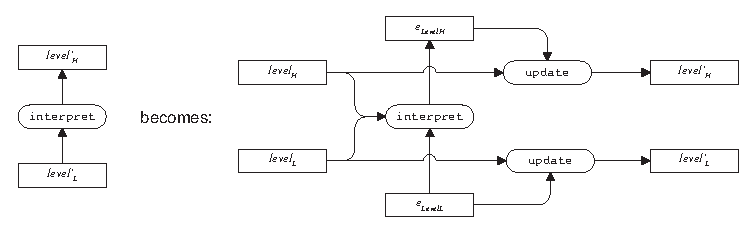
\epsfig{file=pics/eps/levelMapVsdeltaMap.eps}
\end{center}\caption{Level to level vs. edit operation to edit operation }\label{fromLevelToOp} 
\end{center}
\end{small}
\end{figure}


% there is PRES, which is a level thing, pres, which is incremental, and also presLevel
% pres will work on mappings, presLevel won't. Is this PRES? or do we keep PRES abstract
The arrows going from the higher and the lower level to ${\tt translate}$ in the righthand side of Figure~\ref{fromLevelToOp}, are necessary because in some cases, it is hard to map a lower level edit operation onto a higher level edit operation without reference to the respective data levels. If such a mapping is not available, but there is a non-incremental mapping between levels, then the computation sketched in Figure~\ref{computeOps} can be used to obtain a mapping between edit operations. The figure shows how a function ${\tt translate} :: Edit_{Level_{H}} \rightarrow Edit_{Level_{L}}$ can be constructed when only a function with type ${\tt translate'} :: Level_{H} \rightarrow Level_{L}$  is available. In the figure, the edit operation is applied as an update to the old higher level, using the function ${\tt update}$. A new lower level is then computed by applying ${\tt translate'}$ to the updated updated higher level. Finally, the incremental lower level update is computed by taking the difference of the updated lower level and the original. Of course, this is only a sketch, and the difference function does not exist in general, but for some editors, it will be a feasible solution. In order to allow this kind of computation, ${\tt translate}$ needs the values of the higher and lower level as arguments.

\begin{figure}
\begin{small}
\begin{center}
\begin{center}
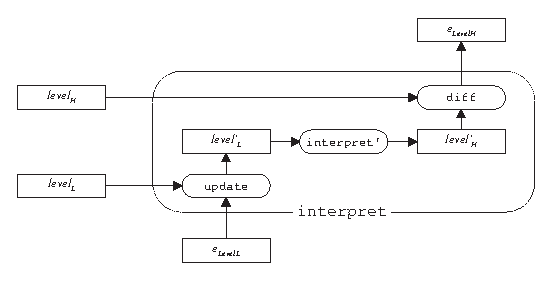
\epsfig{file=pics/eps/levelMap2deltaMap.eps}
\end{center}\caption{Computation of $e_{H}$ from $e_{L}$}\label{computeOps} 
\end{center}
\end{small}
\end{figure}

For the presentation mapping, a similar computation can be performed. Hence, ${\tt present}$ also needs the values of the two adjacent levels. 

Before we give the invariants for the incremental versions of the layer functions, we introduce a short-hand notation for the ${\tt update}$ functions. Especially for larger computations, these functions clutter the diagrams, due to crossing arrows and the many rather uninformative appearances of ${\tt update}$. In the normal notation, an update $data' = {\tt update}~e_{Data}~data$, for values 
$data, data' :: Data$, is represented as:\\

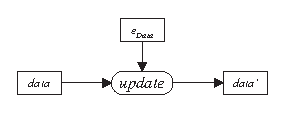
\epsfig{file=pics/eps/updateNotation.eps}

\smallskip
Because an edit operation on a value of type $Data$ can also be regarded as a function of type 
$Data \rightarrow Data$, we use a dashed arrow notation that leaves the function ${\tt update}$ implicit:\\

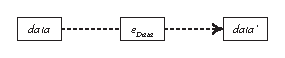
\epsfig{file=pics/eps/updateNotationShort.eps}

Figure~\ref{incrementalTranslate}, shows the righthand side of Figure~\ref{fromLevelToOp} using the new notation.

\begin{figure}
\begin{small}
\begin{center}
\begin{center}
\epsfig{file=pics/eps/translateShortNotation.eps}
\end{center}\caption{Incremental ${\tt translate}$.}\label{incrementalTranslate} 
\end{center}
\end{small}
\end{figure}

\begin{figure}
\begin{center}
\begin{center}
\epsfig{file=pics/eps/maintainESinc.eps}
\end{center}
\caption{**Maintain with es inc.}\label{layerExtraStateInc} 
\end{center}
\end{figure}

**
Now we only need to add reuse, sheets and some arrows to get bla. Also for present.
**


In addition to the extra parameters, and the change from level to edit operation, the equations for the incremental versions of ${\tt present}$ and ${\tt translate}$ also contain a number of explicit ${\tt update}$ functions. Furthermore, note that compared to ${\tt translate}$, the order of the level parameters for         ${\tt present}$ is swapped (ie. first the higher and then the lower level) since the direction of the mapping is also swapped.
 
% PRES and TRANS are not incremental
\begin{small}\begin{math}
{\tt present} :: Sheet_{Pres} \rightarrow  Level_{H} \rightarrow Level_{L}  \rightarrow Edit_{Level_{H}} \rightarrow Edit_{Level_{L}} \\
{\tt translate} :: Sheet_{Trans} \rightarrow  Level_{L} \rightarrow Level_{H} \rightarrow  Edit_{Level_{L}} \rightarrow Edit_{Level_{H}} \\
\text{\{\}}\\
\\
level_{L} = Present~level_{H}\hfill \text{\{Precondition\}}\\
level'_{L} = {\tt update}~e_{Level_{L}}~level_{L}\\
e_{Level_{H}} = {\tt translate}~sheet_{Trans}~level_{L}~level_{H}~e_{Level_{L}} \hfill 
\text{\{\}}\\
level'_{H} = {\tt update}~e_{Level_{H}}~level_{H}\\
level'_{H} = Translate~level'_{L}\hfill \text{\{Intermediate condition\}}\\
\\
level''_{H} = {\tt update}~e'_{Level_{H}}~level'_{H}\\
e'_{Level_{L}} = {\tt present}~sheet_{Pres}~level'_{H}~level'_{L}~e'_{Level_{H}} \hfill 
\text{\{\}}\\
level''_{L} = {\tt update}~e'_{Level_{L}}~level_{L}\\
level''_{L} = Present~level''_{H}\hfill \text{\{Postcondition\}}\\
\end{math}\end{small}

Two updates take place on the higher level, and two on the lower level. However, if we look at Figure~\ref{computeOps}, we can see that a higher level update is performed in the computation of
 ${\tt present}$. Thus, besides $e'_{Level_{L}}$ an implementation of ${\tt present}$ may also return $level''_{H}$. \note{say the the remaining updates disappear because of composition} Similarly, ${\tt translate}$ may return $e'_{L}$. \note{Mention that on composition two of the four updates can be dropped?}

%However, because a layer does not exist on its own, but is composed with other layers (as will be explained 
%in the next Chapter), an adjacent layer will also do an update on the level. Hence


%																
\section{Conclusions}

In one level,  mapping info to higher and lower (except for doc \& rendering), furthermore, the tree can can be regarded bla.

-mapping for pres = Mapping pres. doc only has mapping pres, ren only mapping trans. Core\&extra are wrt mapping of which level is destination. level is extra for pres from higher and trans from lower. Doc only has trans  and ren only pres.



A Proxima Layer:
plaatje met alle in en uitvoer van 1 level


Parse errors in tokens requires trans update on lower. Different model. First research necessary if this way of parsing is good

Proxima offers possibility of solving, not always solution. non tree stuff, or inserted nodes? (redundant parens, tree order) Many problems, need to be solved, but then they can be implemented.




%																
%																
%																
%\section{Bidirectional mappings}
%
%What do we lose exactly by not keeping the mappings
%
%reuse original trees, update mappings upward and downward



%																
%																
%																
%\section{Consequences for each layer}
%Layer examples.
%In arrangement, mappings automatic, formatters etc. rest is easy
%
%In rendering, no mappings
%Doc-Pres, left to editor builder. what happens if we don't do them
%tokens contain origin in edoc. identity is reused. What if type changes?
%
%
%Using caching of parsers and presenters to preserve the mapping
%-- List support for these mappings